\subsection{Current courses page (Roxana)}

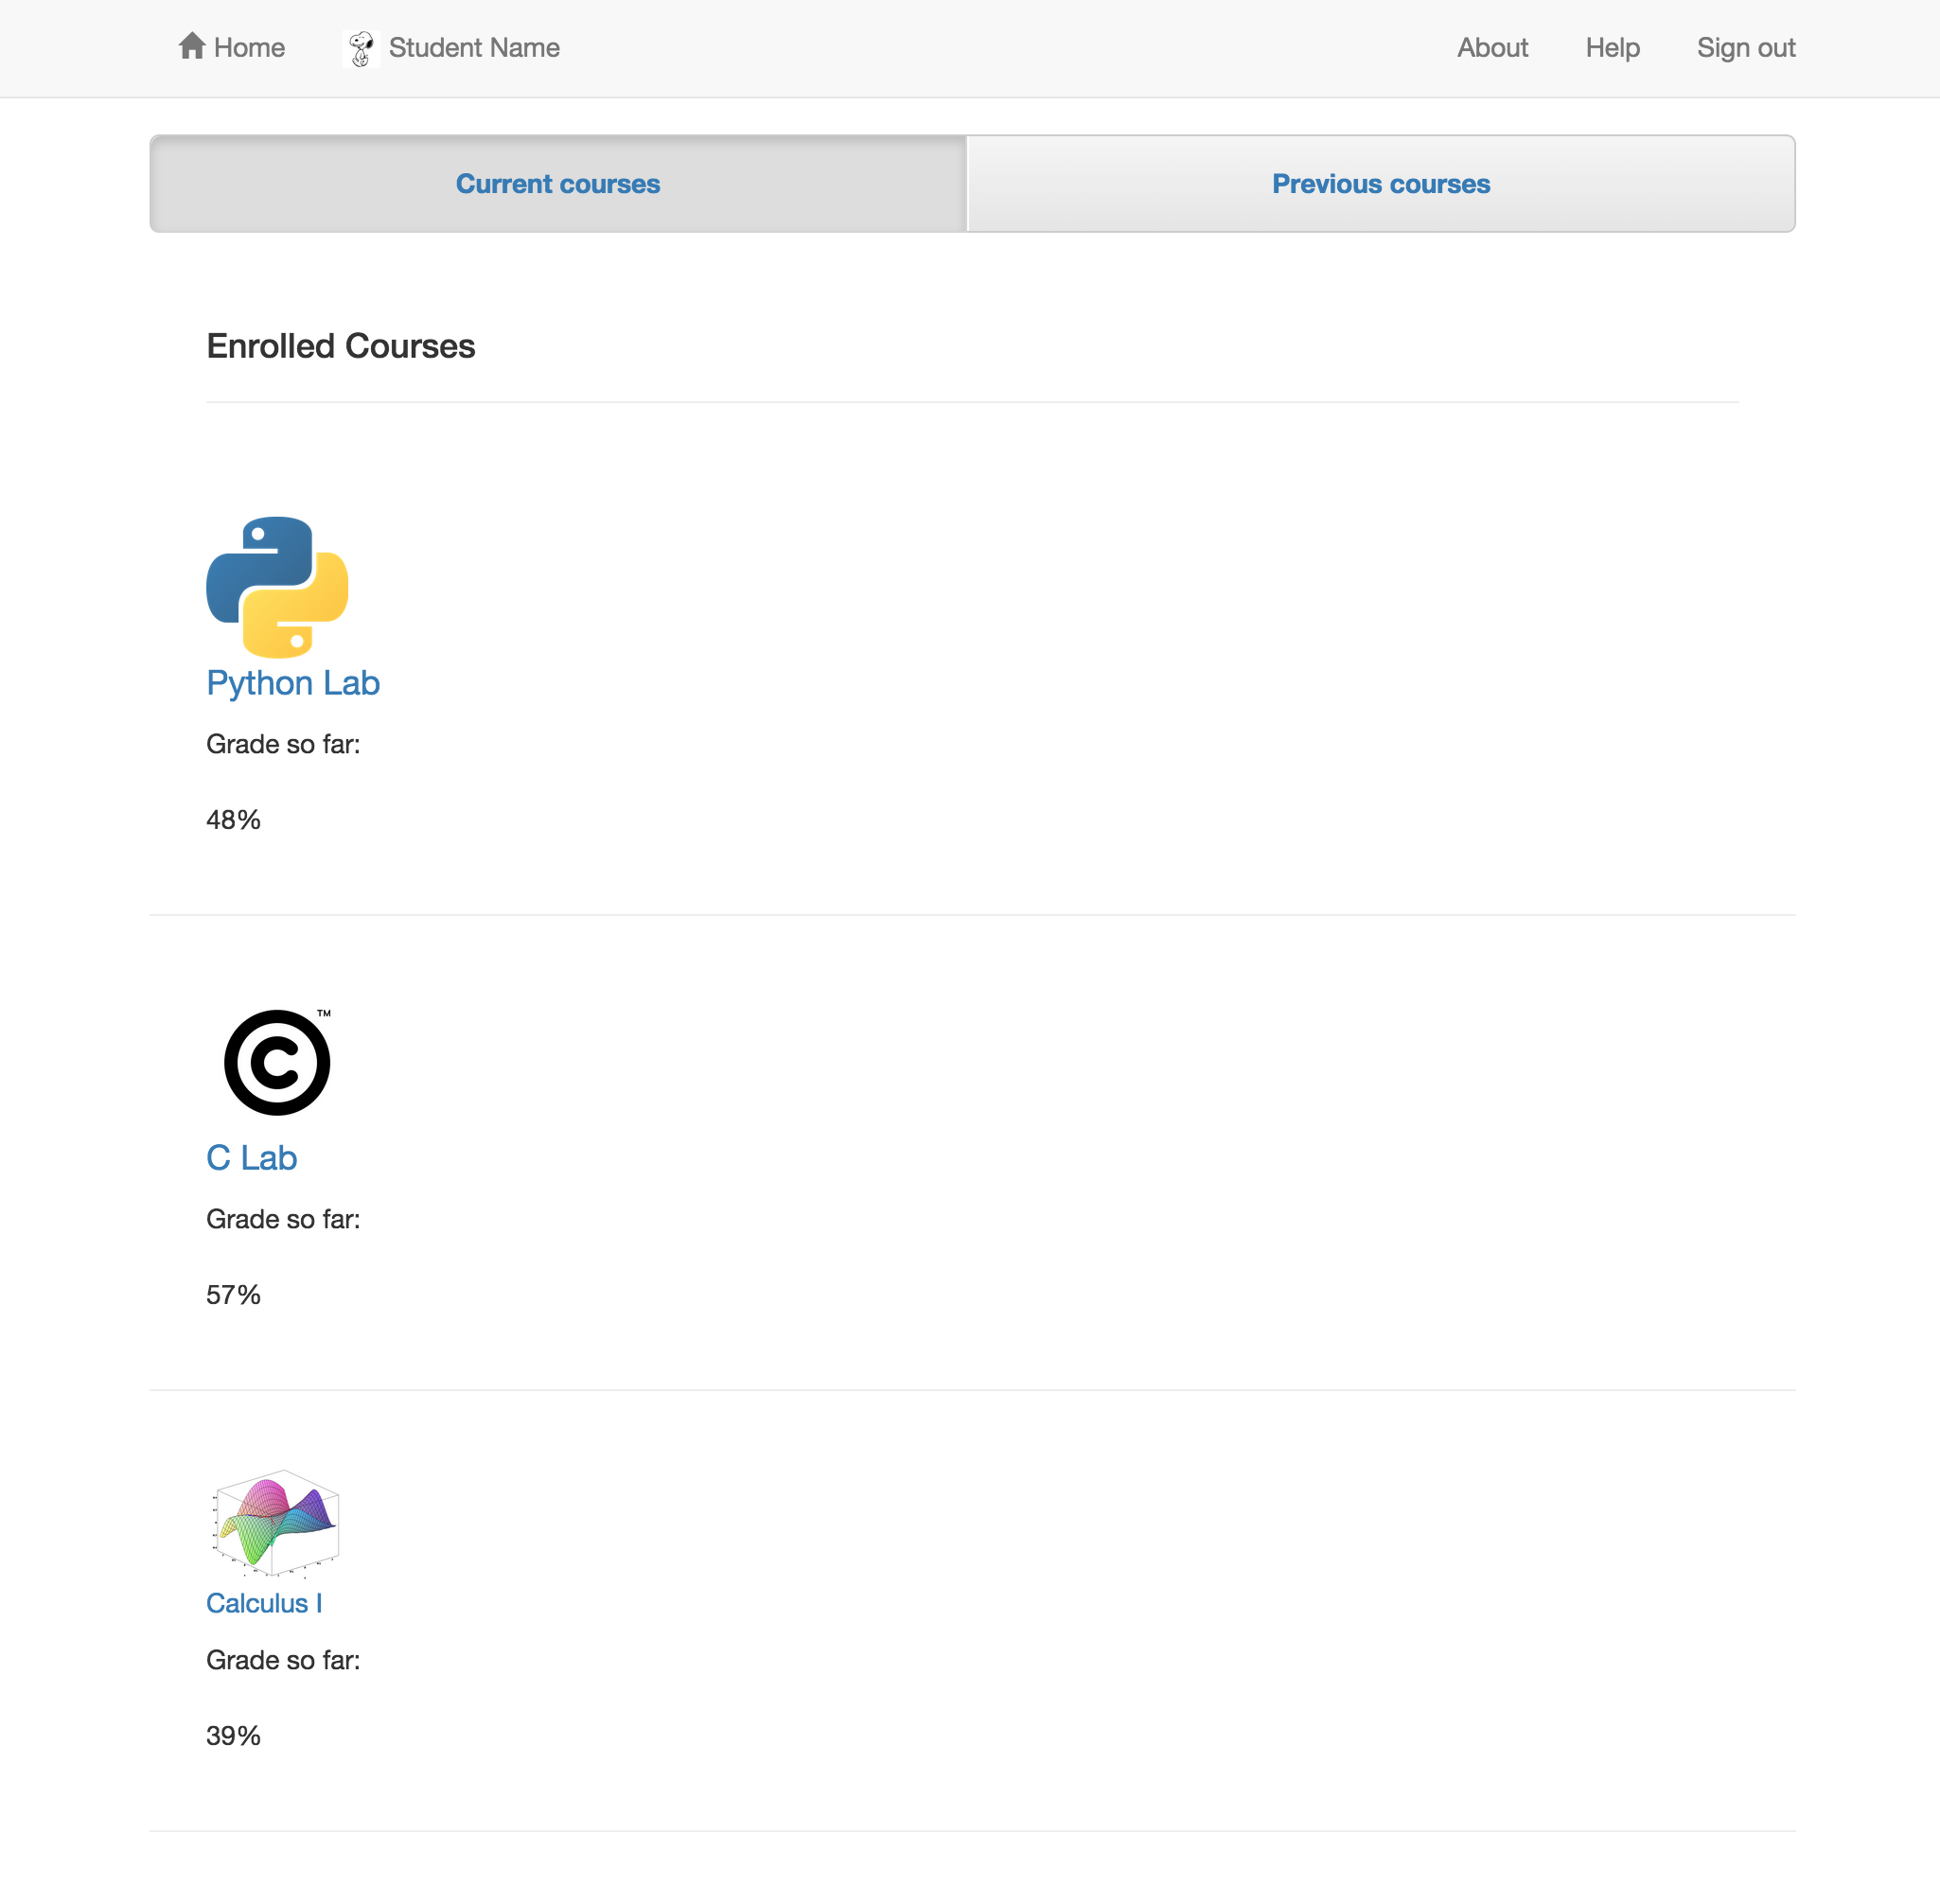
\includegraphics[width=.75\textwidth]{screenshots/CurrentCourses.png}

The previous courses page is very similar in design to the current courses page, with addition of simple marks to indicate whether the student passed or failed the completed course, and a tab bar to navigate through previous semesters.

Orienting the list of semesters horizontally versus the vertical orientation of the courses helps reinforce that the user is navigating through a different set of information than when they simply scroll through courses.

The semester list grows horizontally because it can be compacted better than the list of courses, is less likely to be used, and because it is more difficult to scroll horizontally than vertically on most computers. A less-used feature should use the more difficult action, leaving more natural actions for commonly used features.